\documentclass{article}

\usepackage{import}
\usepackage{pdfpages}
\usepackage{transparent}
\usepackage{xcolor}
\usepackage{amsmath, amsthm, amsfonts, amsthm, mathtools, mathrsfs}
\usepackage{graphicx} 
\usepackage{tikz, tikz-cd} 
\usepackage{hyperref} 
\usepackage[margin=1in]{geometry} 


\newcommand{\R}{\mathbb{R}}
\newcommand{\Q}{\mathbb{Q}}
\newcommand{\Z}{\mathbb{Z}}
\newcommand{\N}{\mathbb{N}}
       %	\newcommand{\incfig}[2][1]{%
%	    \def\svgwidth{#1\columnwidth}
%	    \import{./figures/}{#2.pdf_tex}
%}
%\pdfsuppresswarningpagegroup=1

\newtheorem{prb}{Problem}

\title{MTH 322 Homework 1}
\author{Evan Fox} 
\date{9/17}


\begin{document}
\maketitle

\begin{prb} 
	Proposition 1 details how to construct a equilateral triangle from a given finite line segment.  
\end{prb} 
\begin{proof}
	Given a line segment $AB$, a equilateral triangle is constructed by constructing two circles with radius $AB$ centered at $A$ and $B$ respectivly, 
	then these circles intersect at a point $C$, then it follows since both circles just constructed have the 
	same radius that both line segments $AC$ and $BC$ are congruent to $AB$, then by
	the transitive property, these all have the same length, hence the triangle is equilateral.

	\bigskip

	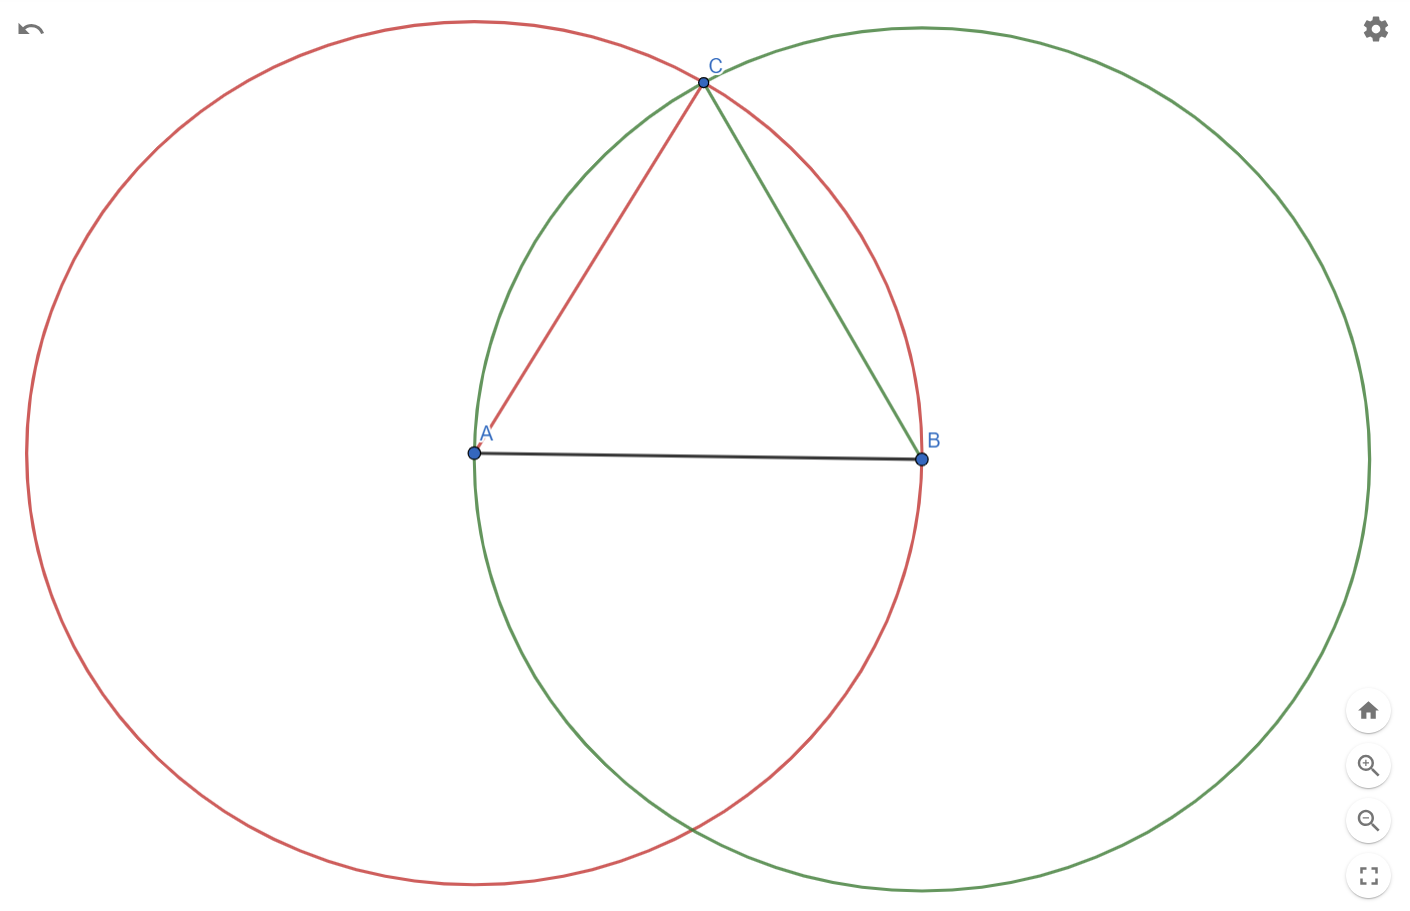
\includegraphics[scale = .5]{equilateral-triangle.png}
\end{proof} 
\noindent I would recomend Euclids method to construct an equilateral triangle because I can think of no simpler method, the proof is very striaghtforward, so it is
easy to see that this process will always yeild the desired result. 


\begin{prb} 

\end{prb} 
\begin{proof} 
	\begin{enumerate}
		\item Consturcting an perp. bisector. 
			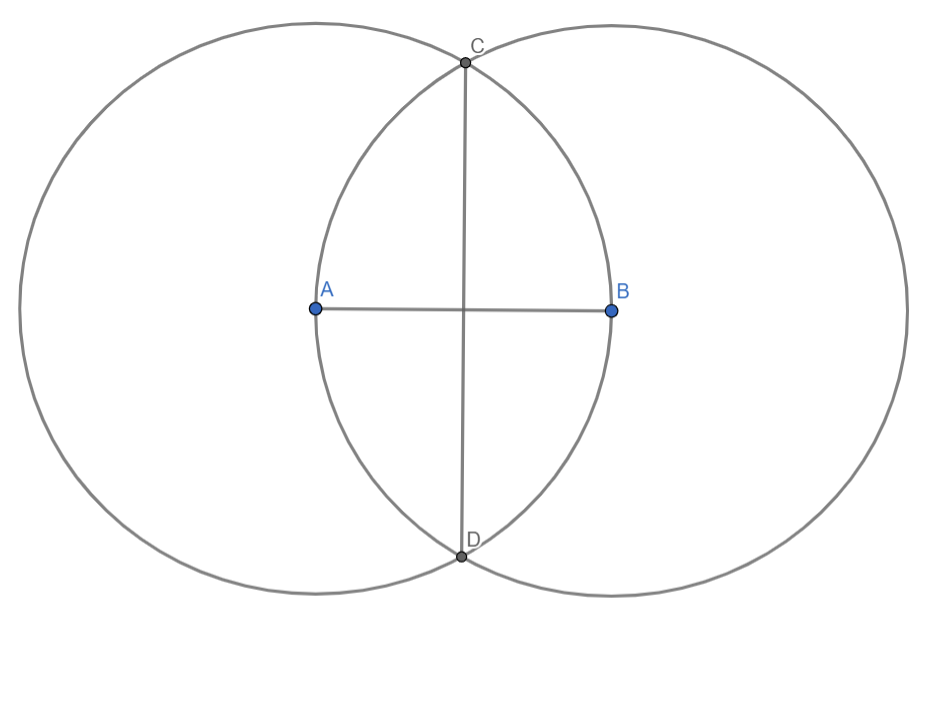
\includegraphics[scale=.25]{BisectLine_prop10.png}
			In order to preform this construction I used prop 10
			in book 1. 
		\item Constructing an angle bisector 
			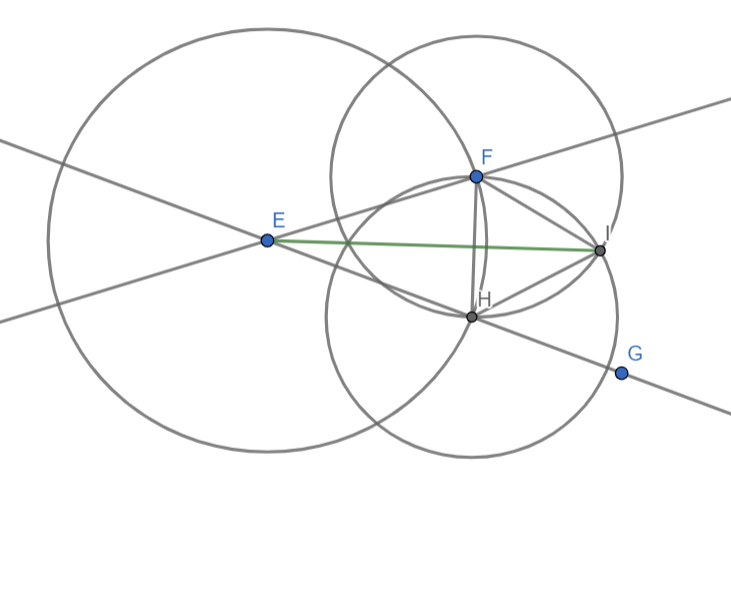
\includegraphics[scale=.25]{AngleBisect-prop9.png}
			This was proposistion 9 in elements book 1. 
		\item constructing  a line parellel to a line $l$ through a 
			point $c$ not on $l$
			\medskip
			\begin{center}

			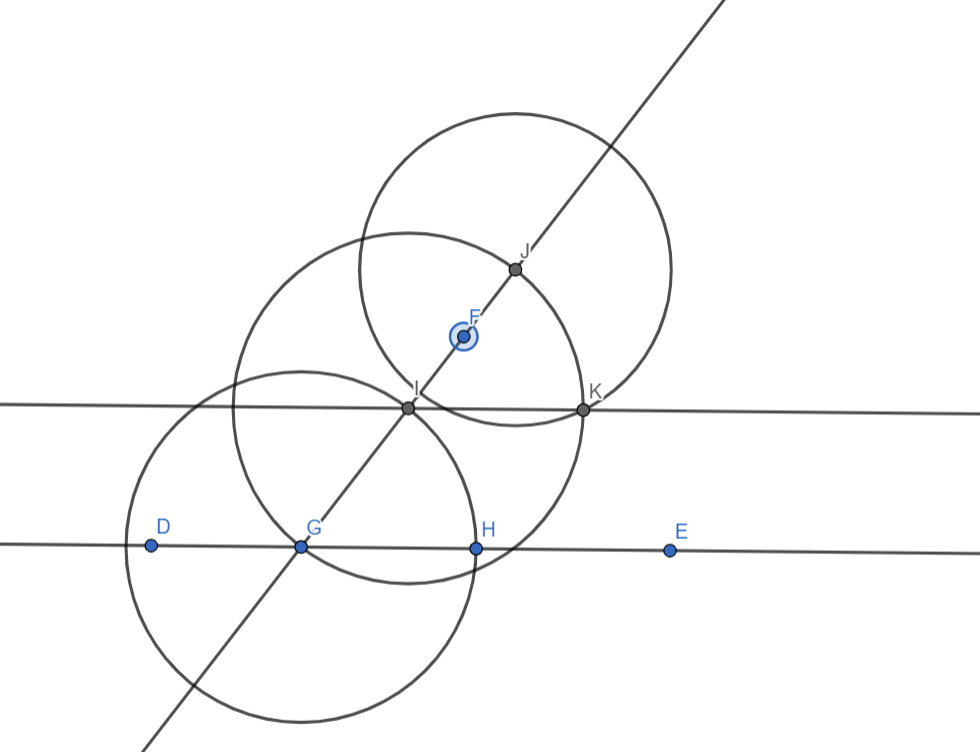
\includegraphics[scale=.25]{ParallelLines_prop31.png}
		\end{center}
			\medskip 

		 The technique comes primarily from proposistion 31 
			in elements book 1. 
		\item Constructing a square of a given side lenth. 
			\medskip
			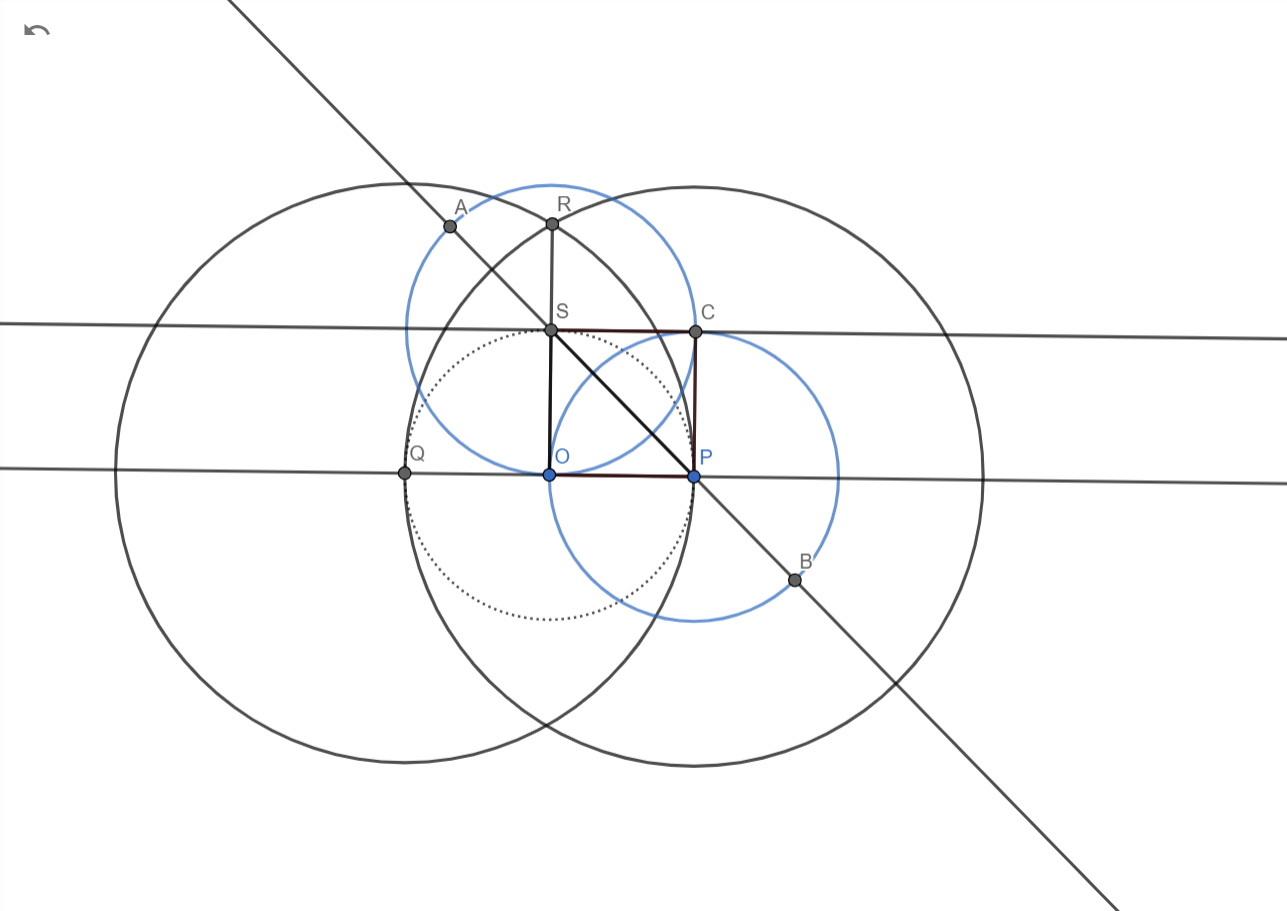
\includegraphics[scale=.25]{squaring_prop46.png}
			\medskip
			This is based on proposistion 46 and prop 31, to 
			construct the parallel lines. 

		\item How to find the center of a circle is given in book 3 
			proposistion 1.
			\medskip
			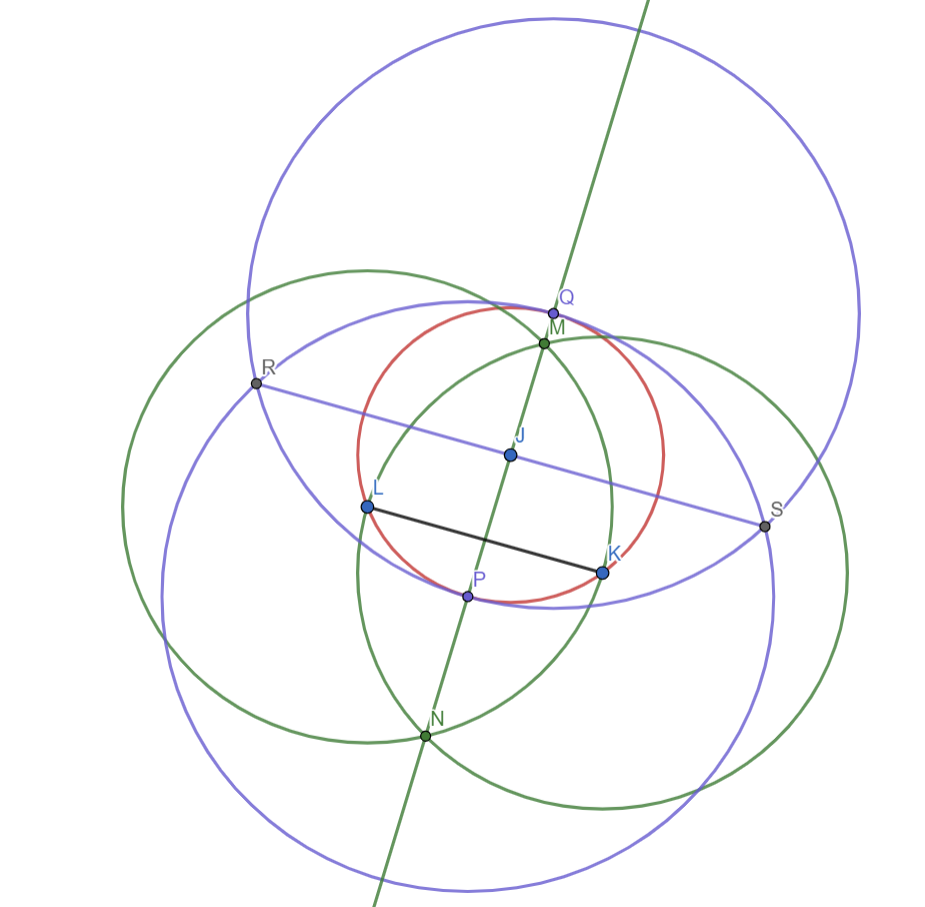
\includegraphics[scale=.25]{CenterofCirc_book3prop1.png}
			\medskip
		The center is given by the intersection of the two 
			differently colored lines.

		\item Proposistion 4 in book 9 says that given two numbers 
			$n, m$ such that $n = a^3$ and $m = b^3$, then there
			exists $c$ such that $mn = c^3$. 
	\end{enumerate}	

\end{proof}

\begin{prb} Library of Alexandria  \end{prb} 
\begin{proof} 
	\begin{enumerate}
	\item Name three mathematicians (at least two of which had connections togeometry) that are mentioned in the video, and the times (minutes and
		seconds) at which each is first mentioned.

		Three mathematicans mentiond are Eratosthenes (2:53), Hypatia (3:56), and Ptolemy (00:56)
	\item What roles do you think or imagine that the Library of Alexandria played
		in the development of geometry or mathematics in general?

		It was probably really imporant so that peoples discoveries could be recoreded and others could access them. With a library, 
		it would be likely that the only way info would travel would be by word of mouth, which would not work well with math. It was definitly 
		a valuable sorce of knowelage for early geomters. 
	\item What really happened to the Library of Alexandria?
		It was not really dystroyed by fire since it was visted by scholars for centrurys after the fire, instead it slowly fell out of 
		favor as changing cultures in the region continually viewed the library as a threat rather than a source of pride. 

	\end{enumerate}

	\medskip 

	\medskip 

	All three loses represent a very sad lose of culture and knoweldge. In the Brazil fire it is estimated that $92$ percent of items where lost. 
	This is a way greater loss than what was lost in the intial fire of the library of Alexandria. Not only this but the Brazil  museum is much larger, 
	the library of Alexandria only had around 400,000 scrolls (which is still alot) but the Brazil museum ost millions of items in its collection. 
	Notre-Damn is a very important place for religious people, since it is a curch unlike the library of Alexandria and the Brazilian Museum. Notre-Damn 
	also contained a large number of artworks and other relics, although I dont think it had many academic texts. 

	\medskip 

	So far in my life librarys have played an important roll as a source of information. When at home I often use my locally library to get work done 
	and at URI I make use of the librarys reascoureses for my school work and for my own interests. Librarys have fostered interest in math in me since I have spent time in the URI library looking at some of the math books and looking for topics that seem interesting. I think the libraries will effect my future life as I intened to be a lifelong learner. 

\end{proof} 

\begin{prb}Thrid problem  \end{prb} 
\begin{proof} 
	
	Some islamic scholars are 
	ukridisi who invented the decimal 
	point, Abul Hasan udlisist who 
	included decimals in a book about 
	arithmitic, and Al -Kashi who also 
	wrote a book about arithmtic using 
	decimal points, which were thought 
	to have been invented in the 1600.

	\medskip 
	I think a big takaway from the 
	video is how many people dont get 
	proper credit for their discoveries 
	and this highlights the importance 
	of studing history so that we can 
	accuratly attribute discoveries to those who have actually discovered it. It was 
	very surprising to see how many supposedly recent discoveries where discovered by 
	people in the east almost a thoushand years ago. 



	\medskip 
	There is value in teaching about 
	the history of geometry (
	and to a greater exent, all math) 
	precisely because there is some 
	dissagrement. This tells us that 
	there are interesting and stimulating
	converesations that can be had. 
	I think the most important 
	principle to follow would 
	be to ensure that you 
	are unbaised and not giving 
	some groups more credit than 
	others. Further, 
	It is important to understand the 
	historical development in order to 
	place the importance of subjects and 
	result accuratly. Not to mention that 
	it helps us to understand our own thought proceses. 

\end{proof} 
\end{document}

